\subsection{\label{sec:calib.ec}Electrocalorimeter Calibration and Resolution}
The timing calibration of the EC system was performed using the ecGammaCal package, using photon hits. This package has been used by multiple running groups, although not all groups. An example of the method, shown in Fig.~\ref{ectall}, compares the photon vertex time according to EC, and the event vertex time. This calibration process uses real photon hits to perform the calibration on a iterative basis by improving the definition of good photon hits using prior calibration constants. Once the preliminary results are obtained, the stability of the calibration constants are monitored on a run-by-run, basis. The integrated results are  shown in Fig.~\ref{ectrunsec} for sector 1 as an example. Clearly, the whole running period can be devided into several stable running periods to obtain the final calibration constants. The quality of the calibration for these individual ranges can be seen in Fig.~\ref{ectrun}. The timing resolution in Fig.~\ref{ectrun} are shown to be about $700$~ps, instead of $500$~ps, due to the fact that in the inclusion of background hits in the EC that are not photons.  

\begin{figure}[h]
\begin{center}
 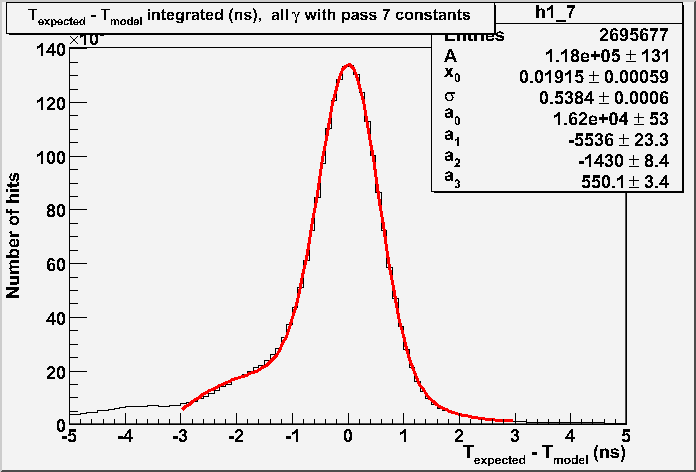
\includegraphics[width=0.9\textwidth]{figures/calib/ec/ec_vtimeall.png}
  \caption{And example of the EC calibration plot, comparing  the difference between photon vertex time according to EC ($T_{model}$, and according to the event vertex time($T_{expected}$), to obtain the EC timing calibration constants. The resolution, integrated for all tubes, are about $500$~ps, for good photon candidates}
  \label{ectall}
  \end{center}
\end{figure}


\begin{figure}[h]
\begin{center}
 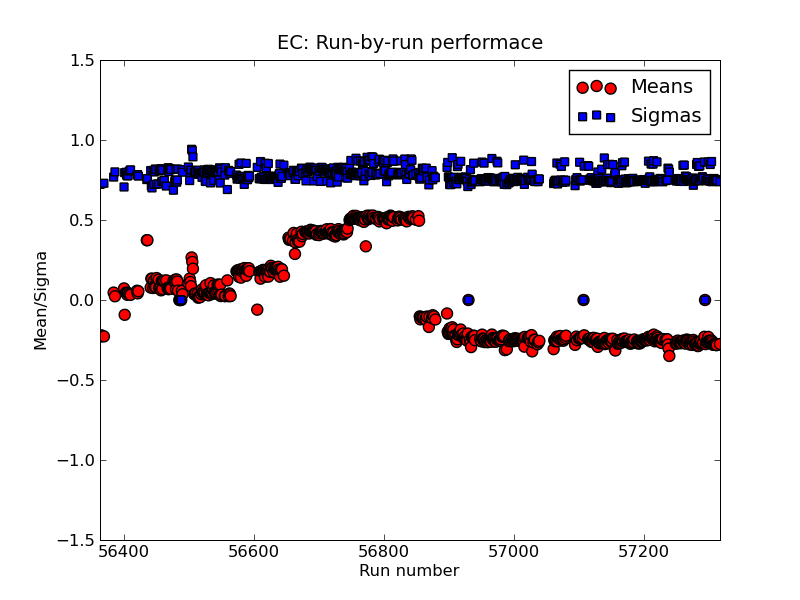
\includegraphics[width=0.9\textwidth]{figures/calib/ec/ec_vtimebyrunsec.png}
  \caption{An example of the ec timing calibration before the final results, i.e., the mean and $\sigma$ of the photon vertex time according to EC, and the event vertex time, as a function of the run numbers. Only sector 1 is shown here.}
  \label{ectrunsec}
  \end{center}
\end{figure}

\begin{figure}[h]
\begin{center}
 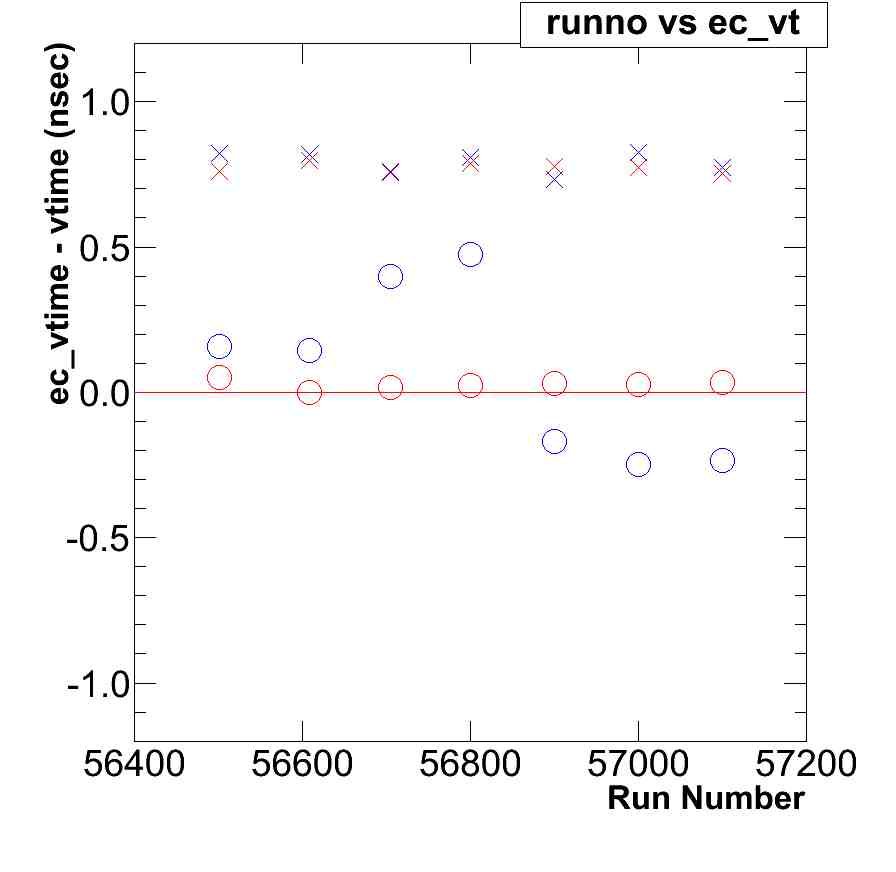
\includegraphics[width=0.9\textwidth]{figures/calib/ec/ec_vtimebyrun.png}
  \caption{The quality of EC timing calibration, i.e., the mean and $\sigma$ of the photon vertex time according to EC, and the event vertex time, monitored for several run ranges. The ranges are chosen according to Fig.~\ref{ectrunsec}. The inclusion of non-photon backgrounds, in the monitoring process, resulted in a larger value of $\sigma$ than the $500$~ps EC timing resolution shown in Fig.~\ref{etcall}. }
  \label{ectrun}
  \end{center}
\end{figure}

Although not solely dependent on the EC timing calibration quality, the $\pi^0$ mass and resolution are also monitored on a run-by-run basis (Fig.~\ref{ecpi0m}$, which shows great stability.

\begin{figure}[h]
\begin{center}
 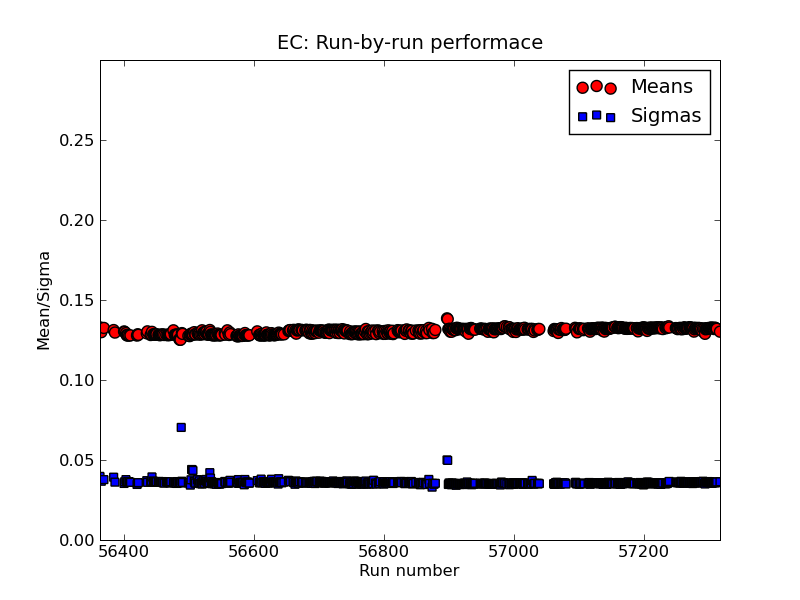
\includegraphics[width=0.9\textwidth]{figures/calib/ec/ec_pi0mass.png}
  \caption{The mass and resolution of the $\pi^0$, reconstructed from fitting two-photon invariant mass spectra, as a function of the run number.}
  \label{ecpi0m}
  \end{center}
\end{figure}

\subsubsection{\label{sec:calib.ec.eff}Electrocalorimeter Efficiency and Bad Paddles}

\FloatBarrier
